% -*- Mode:TeX -*-

%% IMPORTANT: The official thesis specifications are available at:
%%            http://libraries.mit.edu/archives/thesis-specs/

%% The documentclass options along with the pagestyle can be used to generate
%% a technical report, a draft copy, or a regular thesis.  You may need to
%% re-specify the pagestyle after you \include  cover.tex.  For more
%% information, see the first few lines of mitthesis.cls. 

%\documentclass[12pt,vi,twoside]{mitthesis}
%%
%%  If you want your thesis copyright to you instead of MIT, use the
%%  ``vi'' option, as above.
%%
%\documentclass[12pt,twoside,leftblank]{mitthesis}
%%
%% If you want blank pages before new chapters to be labelled ``This
%% Page Intentionally Left Blank'', use the ``leftblank'' option, as
%% above. 

\documentclass[12pt,vi,oneside]{mitthesis}
\usepackage{lgrind}
\usepackage{cmap}
\usepackage[T1]{fontenc}
\pagestyle{plain}

%% Used for displaying images
\usepackage{graphicx}
%% Used for special url fonts
\usepackage{url}
%% Used for mathematical expressions
\usepackage{amsmath}
%% Used for adding captions to tables
\usepackage{caption}

%% Define syntax highlighting
\usepackage{listings}
\usepackage{color}

\definecolor{codegreen}{rgb}{0,0.6,0}
\definecolor{codegray}{rgb}{0.5,0.5,0.5}
\definecolor{codepurple}{rgb}{0.58,0,0.82}
\definecolor{backcolour}{rgb}{0.95,0.95,0.92}
 
\lstdefinestyle{mystyle}{
    backgroundcolor=\color{backcolour},   
    commentstyle=\color{codegreen},
    keywordstyle=\color{magenta},
    numberstyle=\tiny\color{codegray},
    stringstyle=\color{codepurple},
    basicstyle=\footnotesize,
    breakatwhitespace=false,         
    breaklines=true,                 
    captionpos=b,                    
    keepspaces=true,                 
    numbers=left,                    
    numbersep=5pt,                  
    showspaces=false,                
    showstringspaces=false,
    showtabs=false,                  
    tabsize=2
}
 
\lstset{style=mystyle}


% Overwrite some commands
\renewcommand{\contentsname}{Inhaltsverzeichnis}
\renewcommand{\listfigurename}{Abbildungsverzeichnis}
\renewcommand{\listtablename}{Tabellenverzeichnis}
\renewcommand{\bibname}{Bibliografie}
\renewcommand{\chaptername}{Kapitel}
\renewcommand{\figurename}{Abbildung}

\begin{document}

% Define title cover
% -*-latex-*-
% 
% For questions, comments, concerns or complaints:
% thesis@mit.edu
% 
%
% $Log: cover.tex,v $
% Revision 1.8  2008/05/13 15:02:15  jdreed
% Degree month is June, not May.  Added note about prevdegrees.
% Arthur Smith's title updated

% NOTE:
% These templates make an effort to conform to the MIT Thesis specifications,
% however the specifications can change.  We recommend that you verify the
% layout of your title page with your thesis advisor and/or the MIT 
% Libraries before printing your final copy.
\title{my scientific paper}

\author{Yves Beutler}
% If you wish to list your previous degrees on the cover page, use the 
% previous degrees command:
%       \prevdegrees{A.A., Harvard University (1985)}
% You can use the \\ command to list multiple previous degrees
%       \prevdegrees{B.S., University of California (1978) \\
%                    S.M., Massachusetts Institute of Technology (1981)}
\department{BFH Technik und Informatik}

% If the thesis is for two degrees simultaneously, list them both
% separated by \and like this:
% \degree{Doctor of Philosophy \and Master of Science}
\degree{Bachelor of Science BFH in Informatik}

% As of the 2007-08 academic year, valid degree months are September, 
% February, or June.  The default is June.
\degreemonth{Januar}
\degreeyear{2020}
\thesisdate{12. Januar, 2020}

%% By default, the thesis will be copyrighted to MIT.  If you need to copyright
%% the thesis to yourself, just specify the `vi' documentclass option.  If for
%% some reason you want to exactly specify the copyright notice text, you can
%% use the \copyrightnoticetext command.  
%\copyrightnoticetext{\copyright IBM, 1990.  Do not open till Xmas.}

% If there is more than one supervisor, use the \supervisor command
% once for each.
\supervisor{Prof. Dr. Jürgen Vogel}{Betreuender Professor}
\supervisor{Hans Muster}{Experte}

% This is the department committee chairman, not the thesis committee
% chairman.  You should replace this with your Department's Committee
% Chairman.
%\chairman{Arthur C. Smith}{Chairman, Department Committee on Graduate Theses}
%\chairman{ d}{a }

% Make the titlepage based on the above information.  If you need
% something special and can't use the standard form, you can specify
% the exact text of the titlepage yourself.  Put it in a titlepage
% environment and leave blank lines where you want vertical space.
% The spaces will be adjusted to fill the entire page.  The dotted
% lines for the signatures are made with the \signature command.

\maketitle

% The abstractpage environment sets up everything on the page except
% the text itself.  The title and other header material are put at the
% top of the page, and the supervisors are listed at the bottom.  A
% new page is begun both before and after.  Of course, an abstract may
% be more than one page itself.  If you need more control over the
% format of the page, you can use the abstract environment, which puts
% the word "Abstract" at the beginning and single spaces its text.

%% You can either \input (*not* \include) your abstract file, or you can put
%% the text of the abstract directly between the \begin{abstractpage} and
%% \end{abstractpage} commands.

% First copy: start a new page, and save the page number.
\cleardoublepage
% Uncomment the next line if you do NOT want a page number on your
% abstract and acknowledgments pages.
% \pagestyle{empty}
\setcounter{savepage}{\thepage}
\begin{abstractpage}
%% The text of your abstract and nothing else (other than comments) goes here.
%% It will be single-spaced and the rest of the text that is supposed to go on
%% the abstract page will be generated by the abstractpage environment.  This
%% file should be \input (not \include 'd) from cover.tex.
this is a very simple abstract..
\end{abstractpage}

% Additional copy: start a new page, and reset the page number.  This way,
% the second copy of the abstract is not counted as separate pages.
% Uncomment the next 6 lines if you need two copies of the abstract
% page.
% \setcounter{page}{\thesavepage}
% \begin{abstractpage}
% %% The text of your abstract and nothing else (other than comments) goes here.
%% It will be single-spaced and the rest of the text that is supposed to go on
%% the abstract page will be generated by the abstractpage environment.  This
%% file should be \input (not \include 'd) from cover.tex.
this is a very simple abstract..
% \end{abstractpage}

\cleardoublepage

\section*{thanks}

Place your greetings and stuff here.

%%%%%%%%%%%%%%%%%%%%%%%%%%%%%%%%%%%%%%%%%%%%%%%%%%%%%%%%%%%%%%%%%%%%%%
% -*-latex-*-


% Some departments (e.g. 5) require an additional signature page.  See
% signature.tex for more information and uncomment the following line if
% applicable.
% % -*- Mode:TeX -*-
%
% Some departments (e.g. Chemistry) require an additional cover page
% with signatures of the thesis committee.  Please check with your
% thesis advisor or other appropriate person to determine if such a 
% page is required for your thesis.  
%
% If you choose not to use the "titlepage" environment, a \newpage
% commands, and several \vspace{\fill} commands may be necessary to
% achieve the required spacing.  The \signature command is defined in
% the "mitthesis" class
%
% The following sample appears courtesy of Ben Kaduk <kaduk@mit.edu> and
% was used in his June 2012 doctoral thesis in Chemistry. 

\begin{titlepage}
\begin{large}
This doctoral thesis has been examined by a Committee of the Department
of Chemistry as follows:

\signature{Professor Jianshu Cao}{Chairman, Thesis Committee \\
   Professor of Chemistry}

\signature{Professor Troy Van Voorhis}{Thesis Supervisor \\
   Associate Professor of Chemistry}

\signature{Professor Robert W. Field}{Member, Thesis Committee \\
   Haslam and Dewey Professor of Chemistry}
\end{large}
\end{titlepage}



\pagestyle{plain}

  % -*- Mode:TeX -*-
%% This file simply contains the commands that actually generate the table of
%% contents and lists of figures and tables.  You can omit any or all of
%% these files by simply taking out the appropriate command.  For more
%% information on these files, see appendix C.3.3 of the LaTeX manual. 
\tableofcontents
\newpage
\listoffigures
\newpage
\listoftables


% Include your chapters here
\chapter{Sample}

This is just a sample LaTeX template. \cite{YB}
\section{Basics}

We can simply write $code$ inside plain text. \cite[Kap. 1.2]{Bro11}

We should use footnotes\footnote{this is a footnote} as well.

\subsection{Listings}

\begin{enumerate}
    \item enumerations are fancy
    \item some more..
\end{enumerate}

\begin{itemize}
    \item Just an unordered list
    \item add more..
\end{itemize}

\subsection{Images}

We can reference to images like this: \ref{fig:sample}.

\begin{figure}[h!]
    \centering
    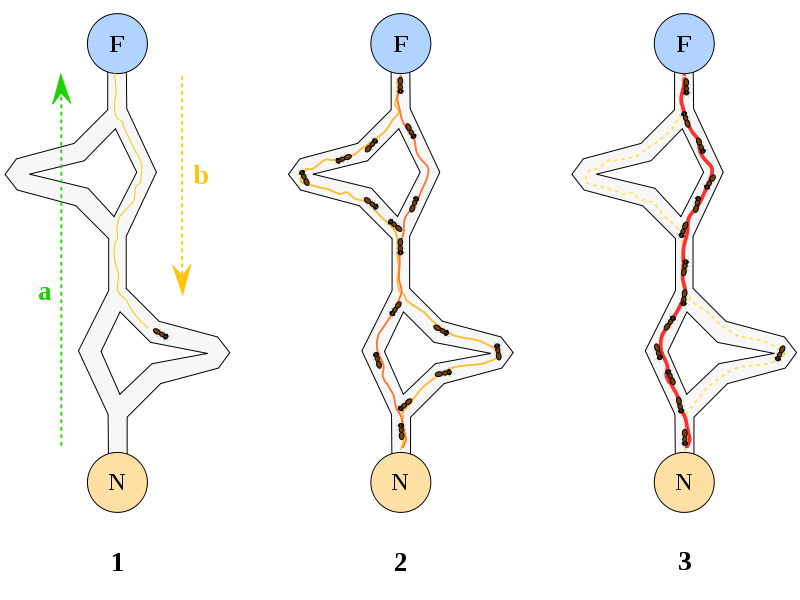
\includegraphics[scale=0.5]{resources/sample.png}
    \caption{this is some sample image \cite{YB}}
    \label{fig:sample}
\end{figure}

\subsection{Maths}

This is some black magic formula:

\begin{equation}
    \label{eq_ant}
    P_{ij}(t) = \begin{cases}
        \frac{[T_{ij}(t)]^\alpha \cdot [N_{ij}]^\beta}
        {\sum_{j \in {allowed}}^{} [T_{ij}(t)]^\alpha \cdot [N_{ij}]^\beta} & \text{wenn } j \in {allowed} \\
        0 & \, \text{sonst}
        \end{cases}
\end{equation}
\label{eq_ant1}

\subsection{Code listings}

We need to define which language to support syntax highlighting.

\begin{lstlisting}[language=Python, caption=Hello World (Python)]
    def hello(name):
        print(f'Hello {name}')
            
\end{lstlisting}

\subsection{Tables}

% \addcontentsline{lot}{table}{This adds the table to the list of tables}
\begin{tabular}{l*{6}{c}r}
    Team              & P & W & D & L & F  & A & Pts \\
    \hline
    Manchester United & 6 & 4 & 0 & 2 & 10 & 5 & 12  \\
    Celtic            & 6 & 3 & 0 & 3 &  8 & 9 &  9  \\
    Benfica           & 6 & 2 & 1 & 3 &  7 & 8 &  7  \\
    FC Copenhagen     & 6 & 2 & 1 & 3 &  5 & 8 &  7  \\
\end{tabular}
\captionof{table}{Champions League Group D}\label{tbl:football}
% \chapter{Evolutionäre Algorithmen}

Diese Subkategorie von Algorithmen wurde durch den natürlichen Prozess der Evolution
inspiriert. Charles Darwin begründete 1838 den Evolutionsprozess und das daraus resultierende
Überleben der jeweils am besten angepassten Individuen durch die natürliche Selektion \cite{Wiki02}.
Diese stellt sicher, dass sich gut an den Lebensraum angepasst Lebewesen in der Natur
durchsetzen können, währenddessen weniger gut angepasste Individuen aussterben. Zudem
arbeitet die Natur nach dem 'Trial and Error' Prinzip. Dadurch werden Mutationen an
Lebewesen ausprobiert und bei positivem Effekt auf das Überleben der Spezies beibehalten,
bei einer Verminderung der Überlebenschancen jedoch wieder rückgängig gemacht. Dieser Prozess
ist sehr zeitaufwändig, jedoch nachhaltig wirksam. Viele Algorithmen wie beispielsweise
der Hill Climbing Algorithmus \cite{Anr18} wenden ebenfalls dieses Prinzip an.

\section{Genetische Algorithmen}

Die Genetischen Algorithmen sind die bekanntesten Vertreter aus der Gruppe der Evolutionären
Algorithmen. Sie orientierten sich an der Populationsgenetik und insbesondere an den Mendelschen
Regeln \cite{Mcc00}.
Bei Genetischen Algorithmen werden häufig Begriffe aus der Biologie verwendet. Die Anzahl an
möglichen Lösungen nennt man Population. Eine einzelne Lösungsvariante wird als Chromosom
bezeichnet, wohingegen diese wiederum aus einer Kombination an Variablen, in der Biologie Gene
genannt, bestehen. Wie aus der Grafik \ref{fig:genetics} zu entnehmen ist, besteht ein Chromosom
$A_n$ aus mehreren Genen.
\\
\begin{figure}[h!]
  \centering
  \includegraphics[scale=0.5]{resources/genetic_algorithms.png}
  \caption{Population, Chromosome und Gene \cite{Mal17}}
  \label{fig:genetics}
\end{figure}

\subsection{Funktionsweise}

Im Folgenden werden die einzelnen Schritte erläutert, welche die Natur wie auch die Genetischen
Algorithmen durchlaufen, um eine Anfangspopulation schrittweise weiterzuentwickeln. Die Natur
sucht nach der erfolgversprechendsten Lösung zum Überleben, wohingegen die Algorithmen
optimale Lösungen für ganz unterschiedliche Problemstellungen suchen. \cite{Mal17}

\subsubsection{Initiale Population}
Eine Population besteht aus mehreren unabhängigen Lösungen, im biologischen Kontext Chromosomen,
um eine bestimmte Problemstellung zu lösen. Bei den meisten Implementationen von Genetischen
Algorithmen wird ein Gen durch einen String repräsentiert. Bei Chromosomen eignen sich auch
Binärwerte um das Vorhandensein eines Gens auszuzeichnen.

\subsubsection{Selektion}
Anhand einer sogenannten Fitnessfunktion wird für jedes Individuum eine Punktzahl berechnet.
Die Punktzahl gibt darüber Auskunft, wie kompetitiv sich ein Individuum gegenüber einem anderen
verhält. Je höher dieser Wert, desto höher sind die Chancen, das besagtes Individuum von der
Selektion für die Reproduktion verwendet wird. Durch die Selektion können nur die fittesten
Individuen ihre Gene an die nächste Generation weitergeben und den schwächeren Individuen wird
der Reproduktionszyklus verwehrt.

\subsubsection{Kreuzung}
Der womöglich zentralste Bestandteil eines Genetischen Algorithmus ist die Kreuzung. Hier werden
aus den zuvor selektierten Individuen, einer Ansammlung der vielversprechendsten Lösungen, zwei
Individuen zur Paarung ausgewählt. Die beiden Ausgewählten tauschen ihre Gene bis zu einem bestimmten
Punkt, dem sogenannten Crossover Point, aus. Die restlichen Gene hinter diesem Punkt werden nicht
verändert. Durch diesen Prozess entstehen gleich zwei neue Individuen.

\subsubsection{Mutation}
Die Natur nutzt Mutationen aus, um die Artenvielfalt innerhalb einer Population zu gewährleisten.
Trotz der geringen Wahrscheinlichkeit kommt es vor, dass einzelne Gene, welche durch die Kreuzung
eigentlich vorhanden wären, nicht mehr vorhanden sind und umgekehrt. Ein Genetischer Algorithmus
flippt beispielsweise einzelne Variablen seiner Nachkommen. Durch die Mutation wird verhindert,
dass unser Algorithmus in einem lokalen Minimum stecken bleibt.

\subsubsection{Terminierung}
Ein Genetischer Algorithmus terminiert, sobald sich die nächste Generation nicht mehr merklich von
ihren Vorgängern unterscheidet. Man spricht oftmals auch von Konvergenz. Es ist jedem Algorithmus
selbst überlassen, wie lange ein Individuum in der Population überlebt. Häufig werden bei jedem
Reproduktionszyklus ein oder mehrere Individuen mit den niedrigsten Fitnesswerten aus der Population
gestrichen. In der Natur übernimmt der Tod diese Funktion.

\subsection{Beispiel Implementation}
Die einzelnen Schritte eines Genetischen Algorithmus sind in Listing A.1 durch
ein Python-Beispiel verdeutlicht. Die verwendete Fitnessfunktion ist sehr rudimentär
gehalten und berechnet lediglich die Summe der vorhandenen Gene. Die Population ist konvergiert,
wenn ein Individuum den Fitnesswert 5 erreicht, sprich alle Gene vorhanden sind.

Zweck dieses Listings ist es, den Ablauf eines Genetischen Algorithmus verständlich darzustellen.
Für eine bessere Übersicht wurden dazu die uninteressanten Teile des Codes gänzlich weggelassen.

\subsection{Vorteile}
Genetische Algorithmen haben gewisse Vorzüge bei der Lösung von komplexen
Problemstellungen gegenüber traditionellen Verfahren. Durch den modularen Aufbau
mit den drei Hauptfunktionen Selektion, Kreuzung und Mutation, lassen sich diese
Algorithmen einfach parallelisieren, was sich in einer besseren Rechenzeit bemerkbar
macht. Weiter generieren sie nicht nur eine Lösung, sondern eine Vielzahl an möglichen
Lösungen, welche mit der Zeit immer bessere Ergebnisse liefern. \cite{Gou19}

\subsection{Anwendungsgebiete}
Es existieren schier endlose Einsatzmöglichkeiten für Genetische Algorithmen. Sie werden unter anderem
zum Trainieren von Neuronalen Netzwerken eingesetzt, zur Berechnung von Fahrplänen wie auch den zu fahrenden
Routen (analog dem Traveling Salesman Problem), zur Konstruktion von Aerodynamischen Fahrzeugchassis in
der Luftfahrt, in der Automobilbranche und häufig auch in der Finanzwirtschaft wie beispielsweise
zur dynamischen Preisberechnung \cite{Tut}.

\section{Genetic Programming}
Eine weitere Unterart der Evolutionären Algorithmen ist Genetic Programming. Ähnlich wie
bei den Genetischen Algorithmen ist Genetic Programming auch von den Mendelschen Regeln
inspiriert worden. Die Population besteht jedoch nicht wie bisher gezeigt aus einzelnen
Lösungen, sondern aus Programmen, welche eine Aufgabenstellung in unterschiedlicher
Qualität lösen können. Ziel ist es, dass diese Programme durch den Vererbungsprozess
von Generation zu Generation besser auf die jeweilige Problemstellung angepasst werden.
\cite{GenGP}

\subsection{Darstellungsformen}
Es stellt sich die Frage, wie eine Applikation repräsentiert werden kann, um anschliessend von
Genetic Programming optimiert werden zu können. Es existieren nebst tree- und stack-basierten
eine lineare sowie eine kartesische Darstellungsform. Im Folgenden wird die tree-basierte Form
genauer erläutert.

\begin{figure}[h!]
  \centering
  \includegraphics[scale=0.5]{resources/genetic_program_tree.png}
  \caption{Einfaches mathematisches Programm als Tree dargestellt \cite{Wiki01}}
  \label{fig:gp_tree}
\end{figure}

Wie in Grafik \ref{fig:gp_tree} erkennbar ist, werden die einzelnen Operationen in der tree-basierten
Darstellungsweise durch Knoten repräsentiert. Die Operanden sind dabei jeweils die Endknoten.
Der Vorteil von einem Tree ist, dass mittels Rekursion sehr simpel über alle Äste iteriert werden
kann. Bei der Kreuzung innerhalb des Genetic Programming Algorithmus werden beispielsweise einzelne
Äste zweier Bäume miteinander kombiniert, um einen komplett neuen Baum zu kreieren. \cite{GenTree}

\subsection{Anwendungsgebiete}
Genetic Programming wird häufig als Machine Learning Tool eingesetzt. Es ist besonders nützlich, wenn
eine Approximation der finalen Lösung genügt, da die Berechnung einer exakten Lösung zu aufwändig
wäre. Ausserdem hilft es in Fällen, wo die genaue Form der Lösung zu Beginn unbekannt ist. Häufige
Einsatzgebiete sind Data Modeling, Feature Selection und Klassifikation.

Es existieren unzählige Beispiele, in denen mit Genetic Programming gleichwertige, wenn nicht sogar
bessere Ergebnisse erzielt wurden als durch einen Menschen. Das Entwerfen von elektrischen
Schaltplänen, KI in Computerspielen, Bilderkennung oder automatisiertes Bugfixing stellen nur einen
kleinen Teil der Einsatzmöglichkeiten dar \cite{Koz10}.


\section{Weitere Algorithmen}
Nebst den beiden behandelten Klassen von Genetischen Algorithmen und dem Genetic Programming existieren
noch weitere Unterarten von Evolutionären Algorithmen. Diese werden hier lediglich aufgelistet, da
eine detaillierte Differenzierung zu den beiden bereits bekannten Algorithmen aus dieser Gruppe den Rahmen
dieser Seminararbeit sprengen würde. Weitere Evolutionäre Algorithmen sind:

\begin{itemize}
  \item Evolution Strategies
  \item Grammatical Evolution
  \item Learning Classifier System
\end{itemize}
% \chapter{Schwarm-Algorithmen}

In der Natur ist es nicht ungewöhnlich, dass sich eine Vielzahl an unabhängigen Individuen
derselben Spezies zu einer Gruppe zusammenschlisst, um überlebenswichtige Aufgaben wie
Nahrungssuche, Umsiedlung oder Fortpflanzung erfolgreich zu meistern. Diese Tierverbände kennen
wir unter vielen verschiedenen Bezeichnungen: Herde, Rudel, Kolonie, Rotte, Kultur, Schule, Sippe
oder Schwarm. Ein Schwarm ist der Inbegriff für eine riesige Ansammlung, zum Beispiel Heringe im Atlantik
oder ein Meer aus Monarchfaltern auf ihrem Weg quer durch Mittelamerika.

Was alle Schwärme auszeichnet ist ihre Schwarmintelligenz. Durch die Kooperation jedes einzelnen,
unabhängigen Individuums wird eine kollektive Intelligenz geschaffen, um auch mit scheinbar
unlösbaren Aufgaben fertig zu werden. Dabei besitzen die einzelnen Individuen bei weitem nicht
einen Bruchteil des Denkvermögens, welches durch den Verbund geschaffen wird. Das durch den Schwarm
aufgebaute Wissen wird durch seine einzelnen Individuen oder die jeweilige Umgebung präserviert
\cite[Kap. 6.1]{Bro11}.

Aufgrund der relativ einfachen Verständnisweise sowie der hohen Effizienz sehen Computerwissenschaftler
grosses Potential in Schwarm-Algorithmen. Daher ist es auch nicht verwunderlich, beteiligen sich seit
den 2000er Jahren viele Wissenschaftler an der Erforschung von Schwarmintelligenz \cite{LL18}.

\section{Ant System}
Der italienische Wissenschaftler Marco Dorigo hat sich mit dem Schwarmverhalten von Ameisenkolonien bei 
ihrer täglichen Futtersuche beschäftigt und 1991 den ersten Ameisenalgorithmus namens Ant System
vorgestellt \cite{Wiki03}.

Sobald Ameisen auf ihrer Futtersuche Nahrung gefunden haben und diese zurück zum Nest transportieren, beginnen
sie, ein bestimmtes Pheromon auszusondern. Der Duftstoff legt sich entlang des zurückgelegten Weges Richtung
Nest ab. Anfänglich schwärmen Ameisen in alle möglichen Richtungen aus. Kürzere Wege zwischen Futterquelle und
Nest sind von den Ameisen stärker frequentiert und weisen eine höhere Pheromonkonzentration auf als
längere Alternativrouten. Zudem neigen Ameisen bei der Wahl des Wegs dazu, den stärker duftenden Weg zu wählen.
Dadurch kreiert die Ameisenkolonie durch ihre Schwarmintelligenz einen sehr kurzen Pfad. Diesen Weg nehmen wir
Menschen meist als Ameisenstrasse wahr \cite[Kap. 6.3]{Bro11}.

\begin{figure}[h!]
    \centering
    \includegraphics[scale=0.45]{resources/swarm_ant_system.png}
    \caption{Funktionsweise des Ant Systems \cite{Wiki03}}
    \label{fig:swarm}
  \end{figure}

In Grafik \ref{fig:swarm} können wir erkennen, dass die Ameisen nach einer gewissen Zeit die Strecken mit den
höchsten Duftstoffkonzentrationen bevorzugen.

\subsection{Funktionsweise}
Möchte man den Ant System Algorithmus implementieren, müssen bestimmte Parameter berücksichtigt werden. Die
Wahrscheinlichkeiten, dass sich eine Ameise am Knotenpunkt $i$ entscheidet nach $j$ zu krabbeln, kann durch
Formel \ref{eq_ant} berechnet werden \cite{Blu03}. 

\begin{equation}
    \label{eq_ant}
    P_{ij}(t) = \begin{cases}
        \frac{[T_{ij}(t)]^\alpha \cdot [N_{ij}]^\beta}
        {\sum_{j \in {allowed}}^{} [T_{ij}(t)]^\alpha \cdot [N_{ij}]^\beta} & \text{wenn } j \in {allowed} \\
        0 & \, \text{sonst}
        \end{cases}
\end{equation}
\label{eq_ant1}

Der interessanteste Part dieser Formel stellt die Pheromonverteilung [\ref{eq_pheromon}] dar. Sie liefert den Wert
für die Pheromonkonzentration zwischen Knoten $i$ und $j$. Die Pheromonintensität ergibt sich
aus dem vorgängigen Durchlauf $(t-1)$ und den aktuell durchgelaufenen Ameisen $\Delta T_{ij}(t, t+1)$. Sie
unterliegt einem zeitlichen Zerfall, auch Evaporation genannt. Dieser Koeffizient $\rho$  stellt sicher, dass
die Pheromonkonzentration nicht ins Unendliche ansteigen kann; Dementsprechend sollte auch $\rho < 1$ sein.
Die Pheromonwerte jeder Teilstrecke werden nach jedem Durchgang mittels (\ref{eq_pheromon}) neu berechnet.

\begin{equation}
    \label{eq_pheromon}
    T_{ij}(t + 1) = \rho \cdot [T_{ij}(t)] + \Delta T_{ij}(t, t+1)
\end{equation}
\label{eq_pheromon1}

Nebst der Pheromonverteilung existiert noch eine weitere Komponente, nämlich die Sichtbarkeit der einzelnen
Knoten $N_{ij}$. Ameisen richten sich nicht nur nach der Duftintensität der Strecke, sondern bevorzugen
nebenbei auch kürzere Wege. Die Sichtbarkeit kann ganz simpel als $\frac{1}{d_{ij}}$ berechnet werden. Dieser
Ansatz ist Greedy \cite{Wiki04} und könnte auch durch eine ausgereiftere Heuristik ersetzt werden.

Um nicht die gleichen Knoten mehrfach zu besuchen, wird eine Tabu-Liste eingesetzt. Diese Liste existiert
für jede einzelne Ameise und wird in jedem Durchlauf mit dem aktuell besuchten Knoten erweitert. Folglich
berechnet sich die Liste der erlaubten Knoten aus der Differenz der Liste aller Knoten und der Tabu-Liste,
in (\ref{eq_ant}) als $allowed$ gekennzeichnet.

Durch die Parameter $\alpha \text{ und } \beta$ können die Pheromonverteilung und die Sichtbarkeit
gewichtet werden. Dieses Feintuning kann das Ant System zu einem reinen Greedy-Algorithmus
$(\alpha = 0, \beta = 1)$ oder zu einem Zufallsalgorithmus $(\alpha = 1, \beta = 0)$ verändern.


\subsection{Anwendungsgebiete}
Der Ant System Algorithmus wurde zum Lösen von Kombinationsproblemen entwickelt. Bei diesem Problemtypen
besteht die Schwierigkeit darin, aus mehreren Teillösungen die optimale Kombination zu finden. Die Summe
an möglichen Lösungen übersteigt somit die Kompetenz von traditionellen Pfadsuch-Algorithmen. Wie anfänglich
in Kapitel 1 behandelt, eignen sich Nature-Inspired Algorithmen für diese Aufgaben besonders gut. Da es
sich bei diesen Problemen um heuristische Optimierungsverfahren handelt, kann der Ant System Algorithmus
aber nicht garantieren, jeweils den bestmöglichen Lösungsweg zu finden \cite{Wiki03}.

Mit dieser Art von Kombinationsproblemen beschäftigen sich beispielsweise Logistikunternehmen, um eine
optimale Transportroute zu finden. Weiter kann das Ant System auch zur Konstruktion von Halbleiterplatten
oder bei der Kantendetektion in der Bildverarbeitung eingesetzt werden \cite{Wiki07}.

\subsubsection{Travelling Salesman Problem (TSP)}
Das Problem des Handelsreisenden ist ein bekanntes Beispiel von kombinatorischen Optimierungsproblemen
\cite{Wiki05}. Man versucht eine festgelegte Anzahl Städte zu besuchen, wobei keine Stadt bis auf die
Anfangsstadt mehrfach besucht werden darf. Ziel ist es, einen optimalen Weg zu finden, bei welchem der
Handelsreisende die kleinstmögliche Distanz zurücklegen muss. Das TSP gehört zu den NP-vollständigen
Problemen, daher existiert kein Algorithmus, welcher den optimalen Weg in polynomieller Laufzeit bestimmen
kann \cite{Wiki06}.

\subsection{Erweiterungen}
Das 1991 vorgestellte Ant System wurde mehrfach weiterentwickelt, um sowohl Laufzeit, als auch Effizienz zu
verbessern. Die populärsten Weiterentwicklungen werden hier kurz erläutert.

\subsubsection{Elite Ant System (1991)}
Das Elite Ant System unterscheidet sich nur geringfügig vom ursprünglichen Ant System. Es verwendet eine
angepasste Pheromonverteilungsfunktion \cite{MZ14}. Anders als beim Ant System, bei welchem jede Ameise
die gleiche Menge an Pheromonen ausströmt, existieren sogenannte Elite-Ameisen, welche eine grössere Menge
an Duftstoffen ausströmen und so die Kolonie bei der Pfadsuche wesentlicher beeinflussen. Der
nach jeder Iteration kürzeste Pfad wird als Elitepfad angesehen und die darauf wandernden Ameisen sind
folglich die Elite-Ameisen \cite{BHS99}.

\subsubsection{Rank-based Ant System (1997)}
Eine weitere Erweiterung des Ant System stellt das Rank-based Ant System dar. Nach jeder Iteration werden
die Ameisen anhand von ihrem zurückgelegten Pfad der Länge nach sortiert. Ameisen mit den kürzeren Pfaden
tragen anschliessend verhältnismässig mehr zur Pheromonverteilung bei als solche mit längeren. Zusätzlich
werden nur die Anzahl $\omega$ besten Ameisen für die Berechnung verwendet. Dies verringert die Gefahr, dass
eine hohe Pheromonkonzentration durch viele Ameisen auf dem gleichen sub-optimalen Pfad entsteht
\cite{BHS99}.

\subsubsection{Max-Min Ant System (1999)}
Anders als beim Ant System legt nur die beste Ameise ihre Pheromonspur. Des Weiteren werden die
Konzentrationen pro Teilpfad mit einem Maximum- und Minimum-Wert versehen. So können keine gänzlich
unattraktiven und auch keine zu stark konzentrierten Pfade entstehen. Wenn die beste Ameise eine Teilstrecke
$ij$ nicht passiert hat, ist der dazukommende Pheromonwert als $\Delta T_{ij}^\text{best} = 0$ definiert
\cite{Dor07}.


\section{Bees Algorithm}
Eine Kolonie Honigbienen schwärmt bei ihrer Suche nach Nektar in einem Radius von über 10km in alle Richtungen
aus. Blumenfelder mit einer grossen Menge an Nektar oder Pollen für die Nachkömmlinge, sollen von einer
grösseren Menge Bienen angeflogen werden, als kleinere Felder mit weitaus weniger Nektar oder Pollen. Sogenannte
Erkundungsbienen, welche zur Klasse der Arbeiterbienen gehören, fliegen zufällige Blumenfelder an. Zurück im
Bienenstock evaluieren die Erkundungsbienen die gefundenen Blumenfelder anhand verschiedener Kriterien wie
Nektarmenge oder Distanz zum Bienenstock. Mit einem Wackeltanz kommunizieren die Bienen ihre Ergebnisse mit
der restlichen Kolonie. Aus dem Wackeltanz können die Bienen die Richtung zum Blumenfeld, die zurückzulegende
Distanz und die ungefähre Nektarmenge ableiten \cite{Bro11}.
Diese einzigartige Fertigkeit lässt die Bienenkolonie immer die gerade passende Anzahl an Arbeiterbienen an
Blumenfelder in ihrem Suchradius ausschwärmen.

\subsection{Funktionsweise}

Wie in Listing A.2 zu erkennen ist, wird über eine bestimmte Anzahl Erkundungsbienen iteriert, welche zufällig
in der Landschaft platziert werden. Jede so besuchte Blumenwiese wird mit einem Wert versehen, welcher Auskunft
über ihre Attraktivität liefert. Dies kann mit dem Fitnesswert aus Kapitel \ref{fig:genetics} verglichen werden.
Eine Blumenwiese steht für eine mögliche Lösung, welche jedoch noch optimiert werden kann. Solange die
Abbruchbedingung noch nicht erreicht ist, werden Arbeiterbienen im Recruiting-Prozess für das Sammeln
von Nektar und Pollen rekrutiert. Je attraktiver die Blumenwiese, desto mehr Bienen sendet der Bienenstock in diese
Richtung aus.

Wie in Zeile 7 dargestellt, werden nur die besten Blumenwiesen weiter behandelt. Die dafür rekrutierten Bienen
werden in einem gewissen Radius um die Blumenwiese platziert. Dies entspricht einer lokalen Suche. Landet nun eine
Biene auf einer Blumenwiese mit besserem Rating, so übernimmt diese Biene neu die Rolle als Erkundungsbiene. Wenn
keine Biene eine attraktivere Blumenwiese (oder Lösung) findet, so wird der Suchradius um die initiale Blumenwiese
verkleinert. Dieser Prozess nennt sich auch Neighbourhood Shrinking. Wenn die Blumenwiese inklusive dem ihr zugehörigen
Suchradius keine brauchbaren Lösungen bereithält, wird das gesamte Gebiet nach einer gewissen Zahl an Iterationen
komplett verlassen (Zeile 9).

Damit der Bees Algorithm nicht in lokalen Minima stecken bleibt, werden die Erkundungsbienen, welche die am wenigsten
attraktiven Blumenwiesen gefunden haben, von diesen abkommandiert und abermals zufällig in der Landschaft platziert.
Dadurch führt der Algorithmus neben einer lokalen auch noch eine globale Suche durch \cite{Wiki08}.

\subsection{Anwendungsgebiete}

Der Bee Algorithm kann für Optimierungsprobleme wie das TSP \cite{Wiki05} verwendet werden. Bemerkenswert ist die Tatsache,
dass der Algorithmus für das Load Balancing grosser Serverfarmen von Web Hosting Firmen eingesetzt wird. So werden mit dem
Bees Algorithm einer Region genauso viele Server zur Verfügung gestellt, wie der Hoster entbehren kann. Dabei ist die
Wichtigkeit der Region, welche hier als Blumenwiese agiert, das Hauptmerkmal zur Verteilung. Die einzelnen Server übernehmen
dabei die Rolle der Bienen \cite{You}.

\appendix
\chapter{Code-Listings}

\section{Genetischer Algorithmus}

\begin{lstlisting}[language=Python, caption=Genetischer Algorithmus (Python)]
    class Individual:
      def __init__(self, genes):
          self.genes = genes
          self.fitness_function(genes)
      
      # calculates fitness of each individual
      def fitness_function(self, genes):
          score = 0
          for gene in genes:
              if gene == 1:
                  score += 1
          self.fitness = score
    
    class Population:
        def __init__(self, individuals):
            self.individuals = individuals
        
        def crossover(self, parent_1, parent_2, cross_value=3):
            offspring_1 = parent_1
            offspring_2 = parent_2
            
            # exchange genes below crossover point
            for i in range(cross_value-1):
                gen = offspring_1.genes[i]
                offspring_1.genes[i] = offspring_2.genes[i]
                offspring_2.genes[i] = gen
            
            return [offspring_1, offspring_2]
    
    def genetic_algorithm():
        generation = 1
        population = Population([
            Individual([0, 1, 0, 1, 0]), Individual([1, 1, 0, 0, 0]),
            Individual([0, 1, 1, 1, 0]), Individual([0, 0, 0, 1, 1]),
            Individual([1, 0, 0, 0, 1]), Individual([1, 0, 1, 1, 0])])
    
        while population.get_fittest().fitness < 5:
            # selection
            parent_1 = population.get_fittest()
            parent_2 = population.get_fittest()
    
            # crossover
            offspring = population.crossover(parent_1, parent_2)
    
            # mutation
            offspring = population.mutate(offspring)
    
            # add offspring, remove weakest individuals
            population.grow(offspring)
            population.kill_weakest()
            generation += 1
    
        print(f'Population converged after {generation} generations')
\end{lstlisting}

\newpage
\section{Bees Algorithm}

\begin{lstlisting}[language=Python, caption=Bees Algorithm (Pseudocode) {\cite{Wiki08}}]
for i=1 to num_of_scouts:
    scout[i] = initialize_scout()
    flower_patch[i] = initialize_patch(scout[i])
    
    while stop_condition=FALSE:
        recruitment()
        for i=1 to num_of_best_sites:
            flower_patch[i] = local_search(flower_patch[i])
            flower_patch[i] = site_abandonment(flower_patch[i])
            flower_patch[i] = neighbourhood_shrinking(flower_patch[i])
    
        for i=num_of_best_sites to num_of_scouts:
            flower_patch[i] = global_search(flower_patch[i])
\end{lstlisting}

\clearpage
\newpage

% \include{appb}

% Include bibliography here
%% This defines the bibliography file (main.bib) and the bibliography style.
%% If you want to create a bibliography file by hand, change the contents of
%% this file to a `thebibliography' environment.  For more information 
%% see section 4.3 of the LaTeX manual.
\begin{singlespace}
\bibliography{main}
\bibliographystyle{alpha}
\end{singlespace}


\end{document}
